\chapter{Information Retrieval}

L'information retrieval è un campo dell'informatica che si occupa di memorizzare e identificare documenti.

L'obiettivo è quello di definire un sistema software che permetta di memorizzare una grande quantità di documenti
in un archivio, e un reperimento efficiente dei documenti rilevanti per l'informazioni che necessita un utente.

La \textbf{rilevanza} è una proprietà soggettiva difficile da definire e misurare.

Diversi tipi di sistemi per accedere a informazioni:
\begin{itemize}
  \item Information Retrieval System (Search Engine)
  \item Database Management System (DBMS)
  \item Information Filtering System (Recommender System)
\end{itemize}

Diversi tipi di comunicazione dell'informazione:
\begin{itemize}
  \item \textbf{Pull Technology}: l'utente richiede esplicitamente un'informazione (information retrieval, browsing hypertext, ...)
  \item \textbf{Push Technology}: l'utente è aggiornato automaticamente con informazioni di possibile interesse (recommendation system)
\end{itemize}

I dati sono dei fatti elementari che vanno interpretati per generare l'informazione.
%
\begin{align*}
  \text{Informazione} = \text{Dati} + \text{Interpretazione}
\end{align*}
%
Un sistema di information retrieval interpreta il contenuto di un documento e definisce una rappresentazione formale per ogni documento.
Data una query fornita da un utente genera un ranking di documenti basato sulla rilevanza che hanno rispetto alla query.

\pagebreak

Componenti del sistema:
\begin{itemize}
  \item \textbf{Document collection}: un documento è l'unità di informazione reperibile.
  \item \textbf{Rappresentazione formale}: generazione di un documento surrogato basato sull'output dell'indexing.
  \item \textbf{Query Language}: vengono specificate le condizioni per la selezione dei documenti.
  \item \textbf{Matching Mechanism}: comparazione delle rappresentazioni formali di documenti e della query
\end{itemize}

\begin{figure}[ht]
  \centering
  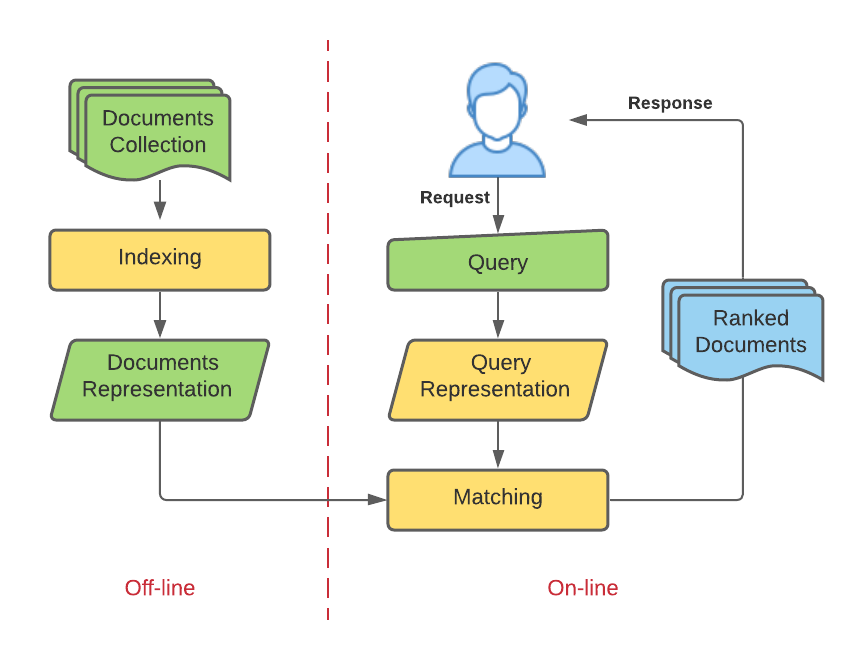
\includegraphics[width=0.8\linewidth]{images/irsystem.png}
  \caption{Schema di un sistema di information retrieval.}
\end{figure}

Un sistema di information retrieval è basato su un modello matematico che fornisce una descrizione formale del documento, della query e
di come comparare le rappresentazioni della query e del documento per stimare la rilevanza.

L'indicizzazione è un processo basato sull'estrazione di elementi (feature) che descrivono (rappresentano) il documento.
Nel caso di testi gli elementi sono generalmente parole e sono prendono il nome di indici.

Il matching può essere:
\begin{itemize}
  \item Esatto (binario): rilevante o non rilevante
  \item Parziale (graduale): la comparazione tra le rappresentazioni ha una certa tolleranza ai mismatch.
\end{itemize}

Per gestire l'informazione in modo automatico bisogna considerare due fattori:
\begin{itemize}
  \item \textbf{Efficienza}: come l'informazione viene rappresentata e processata.
  \item \textbf{Efficacia}: il modo in cui l'informazione viene sintetizzata e come la rappresentazione mantiene il significato originale.
\end{itemize}

Per misurare l'efficienza di un sistema di information retrieval è possibile calcolare precision e recall per ogni query.

\begin{figure}[ht]
  \centering
  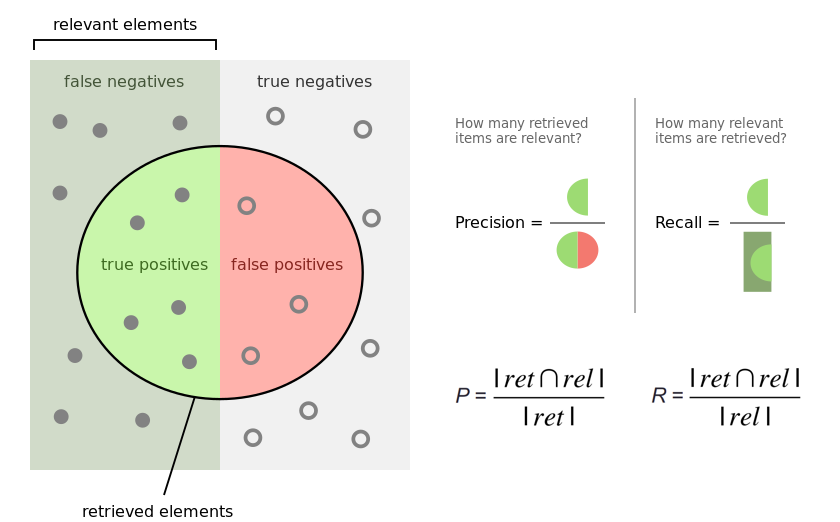
\includegraphics[width=\linewidth]{images/precisionrecall.png}
  \caption{Rappresentazione di precision e recall \cite{wiki:PrecisionRecall}.}
\end{figure}
\bigskip

\begin{quote}
  “IR must try to satisfy information needs expressed in a
  vague, inaccurate way through the ambiguities of the
  natural language, and must compare them, in an
  approximate way with the information contained in a
  document, and expressed through the same natural
  language”\par\nobreak\smallskip\hfill --- Smeaton, 1997
\end{quote}

L'information retrieval è caratterizzata da:
\begin{itemize}
  \item \textbf{Incompletezza} nella rappresentazione dei documenti
  \item \textbf{Soggettività} nel concetto di rilevanza
  \item \textbf{Ambiguità} nel significato dei termini
  \item \textbf{Vaghezza} nelle richieste dell'utente
  \item \textbf{Incertezza} della correttezza dei risultati
  \item \textbf{Approssimazione} del meccanismo di matching
\end{itemize}

\section{Data Structures}
L'indexing automatico di un documento testuale è un processo che mira ad associare gli indici a un testo.

L'uso di indici rende la ricerca efficiente.

L'insieme di tutti gli indici estratti costituiscono il dizionario della collezione.

indexing = index term

Gli indici vengono organizzati in una struttura dati.

Costruzione off-line, accesso ottimizzato al dizionario

Gli index-term che costituiscono il dizionario del documento sono organizzati e memorizzati in un file ad hoc.
Ogni termine punta a una lista che contiene le reference ai documenti di cui il termine è un index.

Dictionary e Posting File

\subsection{Posting File Optimization}

\subsection{Dictionary Organization}
